% Chapter 3

\chapter{Value Analysis} % Main chapter title
\label{chap:Chapter3} % For referencing the chapter elsewhere, use \ref{chap:Chapter3}

In order to develop a new product there is a need for a value analyzing in order to properly assess the relation between cost and value.
This analysis is presented in the following subsections.

\section{New Concept Development Model}

The \gls{NCD}\cite{koen2001providing} is a methodology that supplies a structure to transform an opportunity in a concept by following its key stages.
This will help understand the opportunity value in a well defined manner.

The five key stages, that compose the model defined by Koen\cite{koen2001providing}, were used to define the opportunity behind this project.

\begin{itemize}
    \item \textbf{Opportunity identification} - The opportunity was identified by a member of the deaf community.
    He claimed that there were no solutions to help the process of explaining a given concept using sign language.
    The lexicon of \gls{LGP} is quite small so most words don't have a direct translation, therefore it is required to use the available gestures to explain them.

    \item \textbf{Opportunity analysis} - When analyzing the market, the only tools that have some similarities are the sign language dictionaries but they have some limitations that make it impossible to be a viable solution.
    One of these limitations is that a translation to be added requires that a person is recorded performing the signs required to reproduce the word or expression.
    Another limitation of those dictionaries is the lack of translations for word from the scientific domain.

    \item \textbf{Idea creation} - In this stage, some ideas were formulated for a solution that targets the identified opportunity and is a better fit over the other alternatives analyzed.
    One idea is that the solution to be developed makes the process of explaining a concept automatic.
    For this, the explanation can be found somewhere online and it is possible to obtain it using information retrieval, information extraction and text mining techniques.
    To make the obtained explanation viable to be presented to a member of the deaf community it would be better to translate it to \gls{LGP}.
    For this, there is another GILT project that is already capable of performing this translation and the \gls{API} behind it can be used in this solution.

    \item \textbf{Idea selection} - In this stage, the goal was to take all the possible ideas and approaches into a single one that fulfills the necessary requirements.
    The resulting idea is to develop an automatic interpretation system having the needs of the deaf community in mind.
    This system will use Information retrieval, information extraction and text mining to generate the explanation of a given word or expression.
    It will also translate said explanation to \gls{LGP}.

    \item \textbf{Concept definition} - After having the idea selected, the next step is to define the objectives needed to achieve it.
    The goals of this project are to develop an \gls{API} capable of generating the explanation of a given concept and a web application that will use this, and another \gls{API} to help the deaf community in the process of concept explanation.

\end{itemize}

\section{Value}

The perceived value is based on the benefits and sacrifices identified.

\begin{table}[H]
\caption{Perceived Value}
\label{tab:pValue}
\centering
\begin{tabular}{|m{3cm}|m{3cm}|m{3cm}|m{3cm}|}
\hline
\tabhead{} & \tabhead{Product} & \tabhead{Service} & \tabhead{Relationship} \\
\hline
Benefit & Knowledge & Utility & Trust\\
\hline
Sacrifice &  & Search costs & \\
\hline
\end{tabular}
\end{table}

\section{Value Proposition}

With the goal of helping the process of concept explanation, with focus on the inclusion of the deaf community, this solution aims to use information retrieval, information extraction and text mining techniques to develop a system capable of generating an explanation of a given word or expression and also provide the \gls{LGP} translation.

\section{Business Model Canvas}

In order to ensure a solid structuring of the various business characteristics, it's necessary to use tools that help in the strategic management planning.
The tools to be used must help answer some question, such as:

\begin{itemize}
        \item Who are the clients?
        \item What do they value?
        \item How can we reach them?
        \item What skills are required?
        \item What are the costs associated with our solution?
\end{itemize}

One of the tools that is able to help in this is the Business Model Canvas\cite{osterwalder2010business}, that provides 9 key blocks to aid in the process of planning the business concepts.
The 9 key blocks are:

\begin{itemize}
    \item \textbf{Key Partners} - Describes the network of suppliers and partners that make the business model work.
    \item \textbf{Key Activities} - Describes the most important things a company must do to make the business model work.
    \item \textbf{Key Resources} - Describes the most important assets required to make a business model work.
    \item \textbf{Value Propositions} - Describes the bundle of products and services that create value for the Customer Segments.
    \item \textbf{Customer Relationships} - Describes the types of relationships a company establishes with the Customer Segments.
    \item \textbf{Channels} - Describes how a company communicates with and reaches its Customer Segments to deliver a Value Proposition.
    \item \textbf{Customer Segments} - Defines the different groups of people or organizations a company aims to reach and serve.
    \item \textbf{Cost Structure} - Describes all costs incurred to operate a business model.
    \item \textbf{Revenue Streams} - Represents the money a company generates from each Customer Segment.
\end{itemize}

In Figure~\ref{fig:CANVAS} it is illustrated the Business Model Canvas created for this project.

\begin{figure}[H]
\centering
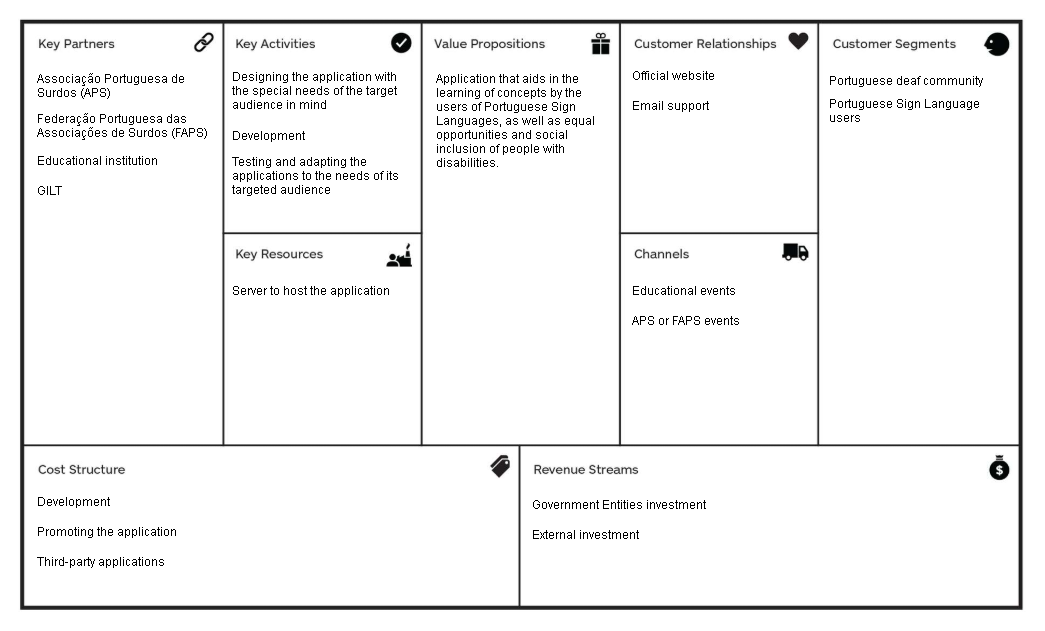
\includegraphics[width=\textwidth,keepaspectratio]{ch3/assets/CANVAS.png}
\caption[Canvas Model]{Canvas Model}
\label{fig:CANVAS}
\end{figure}

The solution developed has two customer segments, which are the Portuguese deaf community and the Portuguese Sign Language users.

As for the product to be provided to this customers, it will be an application that aids in the learning of concepts by the users of Portuguese Sign Language.
By doing so it will help to provide equal opportunities and social inclusion of people with disabilities.

To reach the target audience it should be presented in educational events and in events of the Portuguese Deaf Association or the Portuguese Federation of Deaf Associations.

The customers can expect to find this solution on a website, with all the information needed and the possibility to clarify any doubts through the email support.

In regards to the revenue this solution can get, it will have its origins in the investment made by External companies or Government Entities.

When it comes to the resources required, the most important is the server to host the application to ensure maximum availability.

To increase the chances for the solution to succeed, it is priority to design and develop the application with the special needs of the target audience in mind.
As well as testing and adapting the solution if/when their needs fail to be met.

This solution is in the best interest of education institutions, the Portuguese Deaf Association, the Portuguese Federation of Deaf Associations and GILT so they will be the key partners.

Finally, the costs will have their origin in the development and promotion of the application as well as any third-party application required to be used while escalating the solution.

\section{Analytic Hierarchy Process (AHP)}

The \gls{AHP} was introduced by Saaty\cite{saaty1987analytic} and is an efficient tool to use in the process of complex decision making.
It allows to define priorities using qualitative and quantitative criteria to help reduce complex decisions to a series of paired comparisons.
Using this method will also reduce the bias in process of choice.

\subsection{Stage 1 - Creating the hierarchical decision tree}

This stage consists in creating the hierarchical decision tree where the criteria and viable alternatives are defined.
In regard to the problem, it goal is to determine which natural language processing tools will provide the most value for the project.
The created hierarchical decision tree is presented in the Figure~\ref{fig:AHP}.

\begin{figure}[H]
\centering
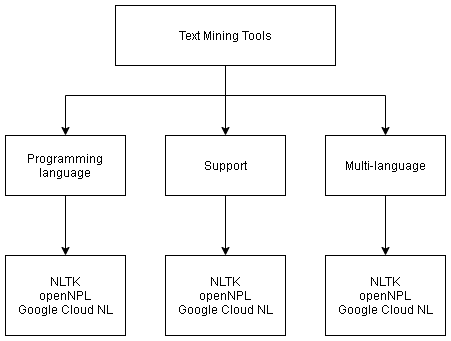
\includegraphics[scale=0.6]{ch3/assets/AHP.png}
\caption[Hierarchical Decision Tree]{Hierarchical Decision Tree}
\label{fig:AHP}
\end{figure}

As observed in the image above, the items of the first layer, corresponding to the primary objectives, had the following criteria behind their selection:
\begin{itemize}
    \item \textbf{Programming language} - The programming language required to be used by the natural language processing tool when developing a solution (e.g. Python, Java, C, JavaScript, etc.).
    \item \textbf{Support} - The number and quality of reliable sources of information about each tool (e.g. Books, Documentation, Forums, etc.).
    \item \textbf{Multi-language} - The compatibility of processing texts and performing tasks using natural languages other than English, with special focus in Portuguese.
\end{itemize}

The presented alternatives in the Figure~\ref{fig:AHP} are the selected natural language processing tools.

NLTK was chosen because it represents a tool that already as a lot of trained models that can be easily used for developing a solution.
The fact that  it's a library for Python, is also important since its the preferred programming language.
Also, as mentioned in Chapter~\ref{chap:Chapter2}, the book available for this tool, allows for a first time user to be able to learn quickly.
Furthermore, after a quick web search its easy to find examples of implementation of text mining approaches using this library.

OpenNLP was chosen because, unlike NLTK, it represents a tool that is meant to be train by the user according to the project needs.
Being a Java library has some relevance since its the second preferred programming language.
The available documentation, that is maintained by the developing community, is not as good as NLTK but it's still easy to follow.

Google Cloud NLP was chosen because, unlike the two upper mentioned, it represents a tool that is not open source and therefore presents payed solutions that may be more efficient.
It can be used with multiple programming languages such as, Python, PHP, Java, Go, etc.
One important aspect of this tools, like other Google services, is the extensive and easy to follow documentation with code snippets that are able to be run in their services to have a better understanding them.

There are countless others tools that are able to perform natural language processing, this were the selected ones since they were heavily recommended and can represent a good portion of them.

The tools here mentioned are described in more detail in Chapter~\ref{chap:Chapter2}.

\subsection{Stage 2 - Alternative and criteria comparison}

This stage consists in defining the priorities between the elements of each hierarchical level.
This is created using the Fundamental scale created by Saaty\cite{saaty1987analytic} that is shown in the Table~\ref{tab:scale}.

\begin{table}[H]
\caption{Fundamental scale \cite{saaty1987analytic}.}
\label{tab:scale}
\centering
\begin{tabular}{|m{4cm}|m{4cm}|m{4cm}|}
\hline
\tabhead{Intensity of importance on an absolute scale} & \tabhead{Definition} & \tabhead{Explanation} \\
\hline
1 & Equal importance & Two activities contribute equally to the objective\\
\hline
3 & Moderate importance of one over another & Experience and judgment strongly favor one activity over another\\
\hline
5 & Essential or strong importance & Experience and judgment strongly favor one activity over another\\
\hline
7 & Very strong importance & An activity is strongly favored and its dominance demonstrated in practice\\
\hline
9 & Extreme importance & The evidence favoring one activity over another is of the highest possible order of affirmation \\
\hline
2,4,6,8 & Intermediate values between two adjacent judgments & When compromise is needed \\
\hline
\end{tabular}
\end{table}

Each comparison between two criterion was defined using the values from the table above, after pondering their relative importance.
The Table~\ref{tab:criteria}, was created to present the result of the comparisons made in regards to the criteria of the decision tree.

\begin{table}[H]
\caption{Comparison Criteria.}
\label{tab:criteria}
\centering
\begin{tabular}{|m{4cm}|m{3cm}|m{3cm}|m{3cm}|}
\hline
\tabhead{Criteria} & \tabhead{Programming language} & \tabhead{Support} & \tabhead{Multi-language} \\
\hline
Programming language & 1 & 1/3 & 1/2 \\
\hline
Support & 3 & 1 & 3 \\
\hline
Multi-language & 2 & 1/3 & 1 \\
\hline
Sum & 6 & 5/3 & 9/2 \\
\hline
\end{tabular}
\end{table}

With the information in the table above it is possible to assess that the criterion "Support" is of moderate importance (3) in comparison with the "Programming language" criterion, and it is of moderate importance (3) when compared to "Multi-language".
Also the criterion "Multi-language" is of slightly more importance (2) when compared to the "Programming language" criterion.

\subsection{Stage 3 - Relative priority of each criterion}

This stage consists in obtaining the normalized criteria values and its relative priorities.
To accomplish this, each value is divided by the sum of its respective column as shown in the Table~\ref{tab:normalization}.

\begin{table}[H]
\caption{Comparison Criteria Normalized.}
\label{tab:normalization}
\centering
\begin{tabular}{|m{4cm}|m{3cm}|m{3cm}|m{3cm}|}
\hline
\tabhead{Criteria} & \tabhead{Programming language} & \tabhead{Support} & \tabhead{Multi-language} \\
\hline
Programming language & 1/6 & 1/5 & 1/9 \\
\hline
Support & 3/6 & 3/5 & 2/3 \\
\hline
Multi-language & 2/6 & 1/5 & 2/9 \\
\hline
\end{tabular}
\end{table}

Having normalized the criteria values, the next step is to calculate the priority order of each criterion.
To accomplish this the arithmetic mean is used in each normalized criterion values previously obtained, as presented in Table~\ref{tab:relativePriority}.

\begin{table}[H]
\caption{Relative priority.}
\label{tab:relativePriority}
\centering
\begin{tabular}{|m{4cm}|m{4cm}|}
\hline
\tabhead{Criteria} & \tabhead{Relative priority} \\
\hline
Programming language & 0.159 \\
\hline
Support & 0.589 \\
\hline
Multi-language & 0.252 \\
\hline
\end{tabular}
\end{table}

With the values from the table above it's possible to conclude that the principal criterion for choosing one of the alternatives is "Support", followed by "Multi-language" and lastly "Programming language".

\subsection{Stage 4 - Consistency evaluation of relative priorities}

This stage consists in calculating the \gls{CR} to assess the consistency of the priorities used in Table~\ref{tab:criteria}.

To calculate the \gls{CR}, the \gls{CI} and the \gls{RI} are used as shown in the following equation:

\begin{equation}
    CR = \frac{CI}{RI}
\end{equation}

It is possible to calculate the \gls{CI} using the Equation~\ref{eqn:CI}.

\begin{equation}
    \label{eqn:CI}
    CI = \frac{\lambda_{max}-n}{n-1}
\end{equation}

In the above equation, $n$ is the number of criteria and $\lambda_{max}$ is the largest eigenvalue of the matrix.

\begin{gather}
    \label{eqn:preLambda}
    \begin{bmatrix}
        1 & 1/3 & 1/2 \\
        3 & 1 & 3 \\
        2 & 1/3 & 1
    \end{bmatrix}
    *
    \begin{bmatrix}
      0.159 \\
      0.589 \\
      0.252
    \end{bmatrix}
      =
    \begin{bmatrix}
      0.481 \\
      1.822 \\
      0.766
    \end{bmatrix}
\end{gather}


\begin{gather}
    \label{eqn:lambdaMax}
    \lambda_{max} =
    \frac{\frac{0.481}{0.159} + \frac{1.822}{0.589} + \frac{0.766}{0.252}}{3}
    = 3.05
\end{gather}

The $\lambda_{max}$ was obtained in the Equation~\ref{eqn:lambdaMax} by calculating the mean of the resulting values from the Equation~\ref{eqn:preLambda} that multiplies the criteria comparison matrix by its priority vector.

The next step is to calculate the \gls{CI} using the following equation:

\begin{equation}
    CI = \frac{3.05-3}{3-1} = 0.025
\end{equation}

The \gls{RI} can be obtained in the index table provided by Saaty\cite{saaty1987analytic}, were a part of it is presented in Table~\ref{tab:index}.

\begin{table}[H]
\caption{Index Table \cite{saaty1987analytic}.}
\label{tab:index}
\centering
\begin{tabular}{|m{1cm}|m{1cm}|m{1cm}|m{1cm}|m{1cm}|m{1cm}|}
\hline
\tabhead{N} & \tabhead{1} & \tabhead{2} & \tabhead{3} & \tabhead{4} & \tabhead{5} \\
\hline
RI & 0 & 0 & 0.58 & 0.90 & 1.12 \\
\hline
\end{tabular}
\end{table}

The \gls{RI} used will be 0.58 since the $n$, as previously is 3.

Having the \gls{CI} and the \gls{RI} values, it was possible to calculate the \gls{CR} as shown in the following equation:

\begin{equation}
    CR = \frac{0.025}{0.58} = 0.043
\end{equation}

Since the obtained value 0.043 is less than 0.1 it is possible to conclude that the values attributed to the properties are consistent.

\subsection{Stage 5 - Construction of the parity comparison matrix for each criterion}

This stage consists in creating a parity comparison matrix for each of the alternatives presented in the hierarchical decision tree, these are the natural language processing tools.
The relative priorities were calculated as shown previously in Stage 3.

\begin{table}[H]
\caption{Programming Language Parity Comparison Matrix.}
\label{tab:progLangPC}
\centering
\begin{tabular}{|m{3cm}|m{3cm}|m{3cm}|m{3cm}|}
\hline
\tabhead{Programming Language} & \tabhead{NLTK} & \tabhead{openNLP} & \tabhead{Google Cloud NL} \\
\hline
NLTK & 1 & 5 & 1/2 \\
\hline
openNLP & 1/5 & 1 & 1/5 \\
\hline
Google Cloud NL & 2 & 5 & 1 \\
\hline
Sum & 16/5 & 11 & 17/10 \\
\hline
\end{tabular}
\end{table}

\begin{table}[H]
\caption{Programming Language Relative Priority.}
\label{tab:progLangPCRP}
\centering
\begin{tabular}{|m{3cm}|m{3cm}|}
\hline
\tabhead{Programming Language} & \tabhead{Relative Priority} \\
\hline
NLTK & 0.354 \\
\hline
openNLP & 0.090 \\
\hline
Google Cloud NL & 0.598 \\
\hline
\end{tabular}
\end{table}

\begin{table}[H]
\caption{Support Parity Comparison Matrix.}
\label{tab:supportPC}
\centering
\begin{tabular}{|m{3cm}|m{3cm}|m{3cm}|m{3cm}|}
\hline
\tabhead{Support} & \tabhead{NLTK} & \tabhead{openNLP} & \tabhead{Google Cloud NL} \\
\hline
NLTK & 1 & 3 & 5 \\
\hline
openNLP & 1/3 & 1 & 3 \\
\hline
Google Cloud NL & 1/5 & 1/3 & 1 \\
\hline
Sum & 23/15 & 13/3 & 9 \\
\hline
\end{tabular}
\end{table}

\begin{table}[H]
\caption{Support Relative Priority.}
\label{tab:supportPCRP}
\centering
\begin{tabular}{|m{3cm}|m{3cm}|}
\hline
\tabhead{Support} & \tabhead{Relative Priority} \\
\hline
NLTK & 0.633 \\
\hline
openNLP & 0.260 \\
\hline
Google Cloud NL & 0.106 \\
\hline
\end{tabular}
\end{table}

\begin{table}[H]
\caption{Multi-language Comparison Matrix.}
\label{tab:multiLangPC}
\centering
\begin{tabular}{|m{3cm}|m{3cm}|m{3cm}|m{3cm}|}
\hline
\tabhead{Multi-language} & \tabhead{NLTK} & \tabhead{openNLP} & \tabhead{Google Cloud NL} \\
\hline
NLTK & 1 & 4 & 1/2 \\
\hline
openNLP & 1/4 & 1 & 1/5 \\
\hline
Google Cloud NL & 2 & 5 & 1 \\
\hline
Sum & 13/4 & 10 & 17/10 \\
\hline
\end{tabular}
\end{table}

\begin{table}[H]
\caption{Multi-language Relative Priority.}
\label{tab:multiLangPCRP}
\centering
\begin{tabular}{|m{3cm}|m{3cm}|}
\hline
\tabhead{Multi-language} & \tabhead{Relative Priority} \\
\hline
NLTK & 0.334 \\
\hline
openNLP & 0.098 \\
\hline
Google Cloud NL & 0.568  \\
\hline
\end{tabular}
\end{table}

To conclude this stage, the hierarchical decision tree was recreated with the all the calculated values, as shown in the Figure~\ref{fig:AHPWeighted}.

\begin{figure}[H]
\centering
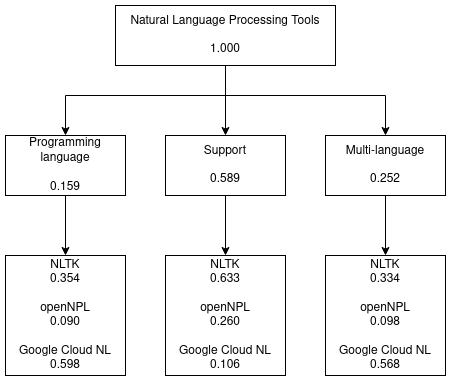
\includegraphics[scale=0.6]{ch3/assets/AHP_weighted.png}
\caption[Hierarchical decision tree with criteria parity comparison]{Hierarchical decision tree with criteria parity comparison}
\label{fig:AHPWeighted}
\end{figure}

\subsection{Stage 6 - Obtain the composite property for alternatives}

This stage consists in obtaining the composite property for the alternatives, to accomplish this, the matrix composed by each criterion relative priority is multiplied by the criteria weight as shown in the following equation:

\begin{gather}
    \begin{bmatrix}
        0.354 & 0.633 & 0.334 \\
        0.090 & 0.260 & 0.098 \\
        0.598 & 0.106 & 0.568
    \end{bmatrix}
    *
    \begin{bmatrix}
      0.159 \\
      0.589 \\
      0.252
    \end{bmatrix}
      =
    \begin{bmatrix}
      \textbf{0.513} \\
      0.192 \\
      0.301
    \end{bmatrix}
\end{gather}

\subsection{Stage 7 - Choice of alternative}

This stage consists in analyzing the obtained values and determine which is the best alternative.
Looking at the obtained values, with the criteria selected and its calculated importance in mind, it is safe to affirm that the best option is NLTK since it obtained the highest valued (0.513).
With the results from this process, the solution to be developed in this project will use NLTK as its natural language processing tool.
